\documentclass[aspectratio=169]{beamer}
\usepackage[T1]{fontenc}
\usepackage[utf8]{inputenc}
\usepackage{tikz}
\usetikzlibrary{tikzmark,shapes,arrows,backgrounds,fit,positioning}

\addtobeamertemplate{navigation symbols}{}{
	\insertframenumber{}
	}

\title{SDEU Baseline}
\author{
  Mauricio Su\'arez Dur\'an and Ioana~C.~Mari\c{s}
}
\institute{IIHE-ULB}

\titlegraphic{
  \begin{figure}[h]
    \centering
   
\includegraphics[width=5cm]{ulbLogo2.png}
    \hspace*{2.cm}
    
\includegraphics[width=5.5cm]{iihe.jpeg}
  \end{figure}
}

\begin{document}
\begin{frame}
  \titlepage
\end{frame}

\begin{frame}
  \begin{itemize}
    \item Baseline stability for pre-production batch of UUBs together with SPMT and SSD in the field.
    \item Data from CDAS: from 01/12/2020 to 21/01/2021
  \end{itemize}
  \begin{figure}
    \centering
    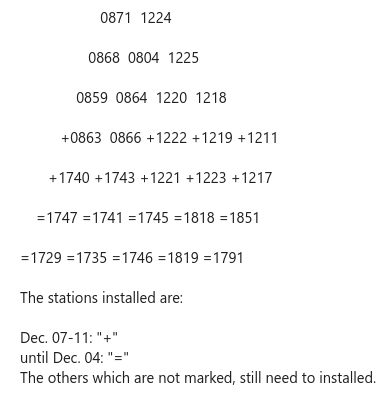
\includegraphics[width=.35\textwidth]{listStations.png}
  \end{figure}
\end{frame}


\begin{frame}
  Distribution of the difference of the mean for the station 1818's PMT1 HG
  \begin{figure}[h]
    \centering
    \includegraphics[width=0.85\textwidth]{../plots/sglEvt.pdf}
	\end{figure}


	\begin{tikzpicture}[overlay,remember picture]
		\path (current page.south west) +(0.1*pi,pi) 
		node[text width=12cm,anchor=south west]{\begin{alignat}{2}
			\mathrm{First\, 100\, bins}  \quad \quad \quad \quad \quad \quad
			\quad \quad \quad \quad  
			\mathrm{Last\, 100\, bins}   \nonumber
		\end{alignat}};
	\end{tikzpicture}

\end{frame}


\begin{frame}
  \centering
  \includegraphics[width=.45\textwidth]{../plots/blPMT1Diffmean100Hg.pdf}\quad%
  \begin{minipage}[b][0.4\textheight][c]{.45\linewidth} \end{minipage}\\[1em]
  \includegraphics[width=.45\textwidth]{../plots/blPMT2Diffmean100Hg.pdf}\quad%
  \includegraphics[width=.45\textwidth]{../plots/blPMT3Diffmean100Hg.pdf}
\end{frame}

\begin{frame}
  Distribution of the difference of the mean for the station 1818's PMT1 HG
  \begin{figure}[h]
    \centering
    \includegraphics[width=1\textwidth]{../plots/blDiffMeanSt1818.pdf}
    \end{figure}
\end{frame}

\begin{frame}
  Distribution of the difference of the mean for the station 1740's PMT1 HG
  \begin{figure}[h]
    \centering
    \includegraphics[width=1\textwidth]{../plots/blDiffMeanSt1740.pdf}
    \end{figure}
\end{frame}

%\begin{frame}
%  \begin{figure}[h]
%    \centering
%    \includegraphics[width=.85\textwidth]{../plots/traces1740.pdf}
%    \end{figure}
%\end{frame}
%
%
%\begin{frame}
%  \begin{figure}[h]
%    \centering
%    \includegraphics[width=.85\textwidth]{../plots/traces1740zoom.pdf}
%    \end{figure}
%\end{frame}
%
%\begin{frame}
%  \begin{figure}[h]
%    \centering
%    \includegraphics[width=.85\textwidth]{../plots/tracesFirstLast1740zoom.pdf}
%    \end{figure}
%\end{frame}


\begin{frame}
	RMS difference for traces that agree with: $\mid \mathrm{Mean}_f - \mathrm{Mean}_l \mid < \left( 2*\mathrm{RMS_f} \right) $

  \centering
	\includegraphics[width=.49\textwidth]{../plots/trOkPMT1Hg.pdf}\quad%
	\begin{minipage}[b][0.4\textheight][c]
		{.45\linewidth}
	\end{minipage}\\[1em]
	\includegraphics[width=.48\textwidth]{../plots/trOkPMT2Hg.pdf}\quad%
	\includegraphics[width=.48\textwidth]{../plots/trOkPMT3Hg.pdf}
\end{frame}


%\begin{frame}
%	RMS Difference
%
%	\centering
%	\includegraphics[width=.7\textheight]{../plots/trOkPMT1Hg.pdf}\quad%
%	\begin{minipage}[b][0.1\textheight][c]
%		{.15\linewidth}
%	\end{minipage}\\[1em]
%	\includegraphics[width=.425\textwidth]{../plots/trOkPMT2Hg.pdf}\quad%
%	\begin{tikzpicture}
%		\node[anchor=south west,inner sep=0] at (1,-3.3) {\includegraphics[width=.425\textwidth]{../plots/trOkPMT3Hg.pdf}};
%		\draw<1>[red,ultra thick,rounded corners] (1.,0.) rectangle (\textheight-2cm,0.3);
%	\end{tikzpicture}
%
%\end{frame}


\begin{frame}
	1851 station's PMT3 HG

  \centering
	\includegraphics[width=.48\textwidth]{../plots/traces1851Pmt3.png}
	\includegraphics[width=.48\textwidth]{../plots/traces1851FLPmt3.pdf}
\end{frame}


\begin{frame}
	Distrubition of RMS for the last 100 bins of station 1851
	\centering
	\includegraphics[width=1.\textwidth]{../plots/rmsDistriPmt1851.pdf}
\end{frame}


\begin{frame}
	Position of VEM-Charge, average per day (traces agree with: $\mid \mathrm{M}_f - \mathrm{M}_l \mid < \left( 2*\mathrm{RMS_f} \right) $)

  \centering
	\includegraphics[width=.49\textwidth]{../plots/chargePMT1Hg.pdf}\quad%
	\begin{minipage}[b][0.4\textheight][c]
		{.45\linewidth}
	\end{minipage}\\[1em]
	\includegraphics[width=.48\textwidth]{../plots/chargePMT2Hg.pdf}\quad%
	\includegraphics[width=.48\textwidth]{../plots/chargePMT3Hg.pdf}
\end{frame}


\begin{frame}
	Position of VEM-Peak, average per day (traces agree with: $\mid \mathrm{M}_f - \mathrm{M}_l \mid < \left( 2*\mathrm{RMS_f} \right) $)

  \centering
	\includegraphics[width=.49\textwidth]{../plots/peakPMT1Hg.pdf}\quad%
	\begin{minipage}[b][0.4\textheight][c]
		{.45\linewidth}
	\end{minipage}\\[1em]
	\includegraphics[width=.48\textwidth]{../plots/peakPMT2Hg.pdf}\quad%
	\includegraphics[width=.48\textwidth]{../plots/peakPMT3Hg.pdf}
\end{frame}


\begin{frame}
	A/P average per day, traces that agree with: $\mid \mathrm{Mean}_f - \mathrm{Mean}_l \mid < \left( 2*\mathrm{RMS_f} \right) $

  \centering
	\includegraphics[width=.49\textwidth]{../plots/apPMT1Hg.pdf}%\quad%
	\begin{minipage}[b][0.2\textheight][c]
		{.15\linewidth}
	\end{minipage}\\[1em]
	\includegraphics[width=.48\textwidth]{../plots/apPMT2Hg.pdf}\quad%
	\includegraphics[width=.48\textwidth]{../plots/apPMT3Hg.pdf}
\end{frame}


\begin{frame}
  \centering
	{\Huge\bf\it Thanks}
\end{frame}


\end{document}
